\chapter{Optimal Control Problem}
\label{Ch:OCP}
%
Once the model is fully formulated the OCP can be build around it. The focus of this thesis is to compute minimum time manoeuvres, therefore the OCP must be constructed following some specific steps depending on the method chosen. In this work the OCP is solved using indirect method through the software PINS \cite{bertolazzi2006symbolic}. In the following section the whole process is explained in details.
%
\section{General OCP}
%
In general the OCP problem is formulated in this way.
%
\begin{equation}
    \begin{aligned}
    &\underset{x(\cdot), u(\cdot)}{\operatorname{minimize}} \quad \mathcal{J}(x(t), u(t), t)\\
    &\begin{aligned}
        {\text { subject to }} \;
        & \mathcal{F}(x^{\prime}(t)x(t),u(t),t)=0, \quad t \in[a, b] \quad \text{(Dynamic System)}\\
        & b(x(a),x(b))=0, \quad \text{(Boundary Conditions)}\\
        & h(x(t),u(t),t)=0, \quad \text{(Equality constraints)}\\
        & g(x(t),u(t),t)>=0, \quad \text{(Inequality constraints)}\\
        & x(t) \in \mathbb{R}^{n_s}, \; u(t) \in \mathbb{R}^{n_c}
    \end{aligned}\\
    \end{aligned}
    \label{eq:GenOCP}
\end{equation}
%
where $\mathcal{J}x(\cdot)$ is the cost function that in general is written like the following.
%
\begin{equation}
    \mathcal{J}(x(t), u(t), t)=\mathcal{M}(x(a), x(b))+\int_{a}^{b} \mathcal{L}(x(t), u(t), t) \mathrm{d} t
\end{equation}
%
$\mathcal{F}(x^{\prime}(t)x(t),u(t),t)=0$ is the general expression for the system of ODE that can also be written in the form
%
\begin{equation}
    A(x(t), t) x^{\prime}(t)=f(x(t), u(t), t)
\end{equation}
%
in which all derivatives of the states appear linearly. Consequently, one can collect the mass matrix $A(x(t), t)$ which is not always invertible. The system of ODE is implicit in this case. This make the direct method hard to use if not impossible.\\
$x(t)$ is the vector of states of dimension $n_s$ and $u(t)$ is the vector of the controls of size $n_c$.
%
The aim of this study is to compute minimum time manoeuvre. Therefore the extremes of integration became $0$ and $T$ instead of $a$ and $b$. Moreover, the model constructed do not need any equality constraints. The lagrange function in this case is simple because of our interest in the minimum time problem.
%
\begin{equation}
    \mathcal{L}(x(t), u(t), t) = 1
\end{equation}
%
This combined with neglecting the Mayer therm $\mathcal{M}(\cdot)$ (most of the time in unnecessary) yields a cost function such as:
%
\begin{equation}
    \mathcal{J}(x(t), u(t), t) = \mathcal{M}(x(a), x(b))+\int_{0}^{T}  \mathrm{d} t = T 
\end{equation}
%
This lead to a simplified version of the problem
%
\begin{equation}
    \begin{aligned}
    &\underset{x(\cdot), u(\cdot)}{\operatorname{minimize}} \quad T \\
    &\begin{aligned}
        {\text { subject to }} \;
        & \mathcal{F}(x^{\prime}(t)x(t),u(t),t)=0, \quad t \in[0, T] \quad \text{(Dynamic System)}\\
        & b(x(0),x(T))=0, \quad \text{(Boundary Conditions)}\\
        & g(x(t),u(t),t)>=0, \quad \text{(Inequality constraints)}\\
        & x(t) \in \mathbb{R}^{n_s}, \; u(t) \in \mathbb{R}^{n_c}
    \end{aligned}\\
    \end{aligned}
    \label{eq:OCPminT}
\end{equation}
%
$T$ is a parameter and the problem cannot be solved in this therm. However there are several techniques to obtain a solvable OCP. The transformation will be discussed in the following sections.
%
\section{Curvilinear Coordinates}
%
\begin{figure}[htb]
    \centering
    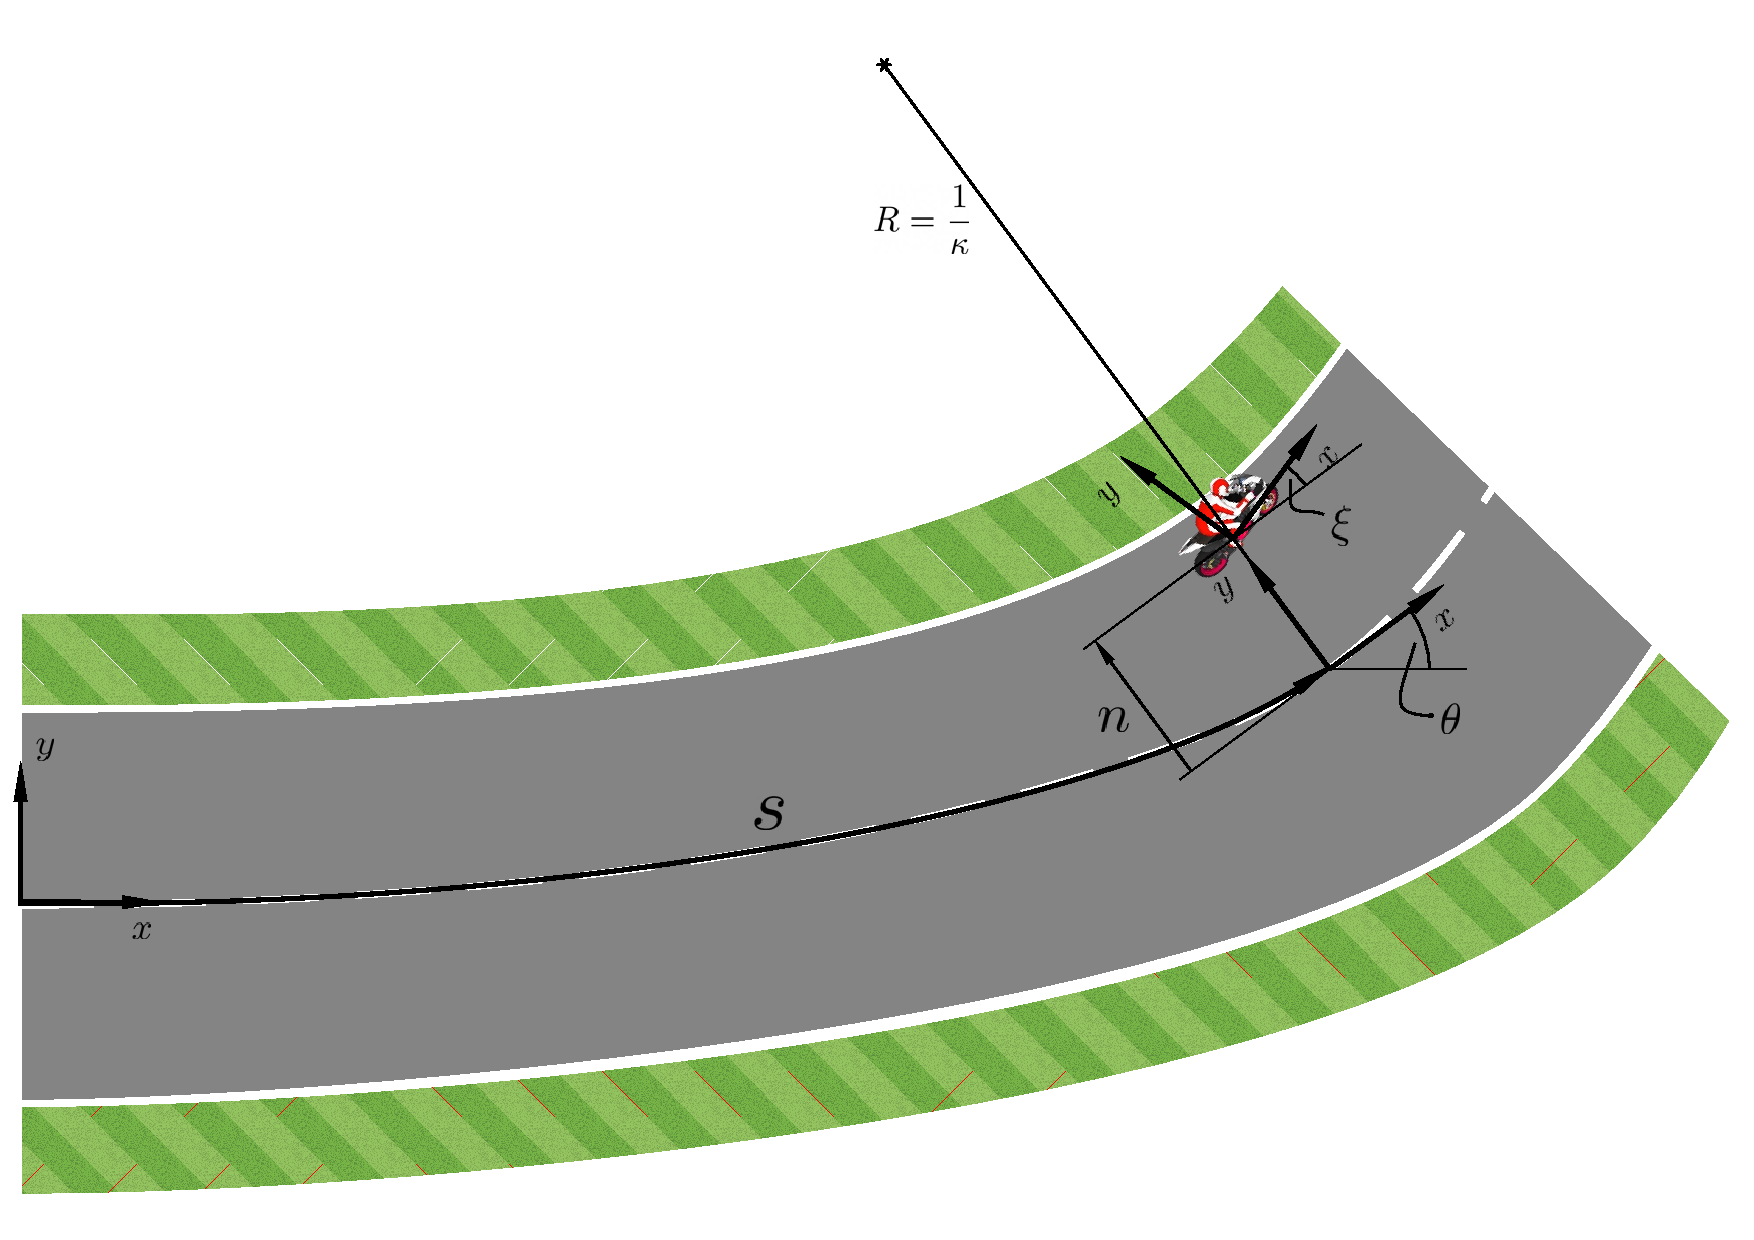
\includegraphics[width=\linewidth]{Coordinates/CurvCoord.pdf}
    \caption{Curvilinear coordinates}
    \label{fig:CurvCoord}
\end{figure}
%
The curvilinear coordinate are a convenient set of coordinate to compute OCPs. This is a well known technique in literature. In this thesis the curvilinear coordinate used consider only a motion on plane (2D). However it can be extended to the three-dimensional space as did by Leonelli and Limebeer \cite{leonelli2019optimal}.\\
%
The curvilinear coordinates ($s(t)$, $n(t)$,$\xi(t)$) can be mapped to quasi states can be obtained defining a reference frame mobile. This is translated with respect to ground of coordinate $\it xm(t)$ and $\it ym(t)$ and rotated around the vertical direction $z$ of an angle $\theta(t)$ (Figure \ref{fig:CurvCoord}).
%
\begin{equation}
\left[ \begin{array}{cccc} 
    \cos \left( \theta \left( t \right) \right) &-\sin \left( \theta \left( t \right)  \right) &0&{\it xm}\left( t \right) \\ 
    \sin \left( \theta \left( t\right)  \right) &\cos \left( \theta \left( t \right)  \right) &0&{\it ym} \left( t \right) \\ 
    0&0&1&0\\ 
    0&0&0&1
\end{array} \right]    
\end{equation}
%
$\theta$ is different from the pitch angle of the previous chapter and will be dropped in the next few passages.\\
From the reference frame previously defined one can define a moving reference frame with longitudinal velocity $\frac {\rm d}{{\rm d}t} s(t)$ and angular velocity $\frac {\rm d}{{\rm d}t} s(t) \kappa(t)$. The last term represent the linear velocity divided by the radius of curvature. In fact $\kappa$ is the curvature of the curvilinear coordinate. $\kappa$ is not a direct function of time. It depends on the curvilinear coordinate $s$, $\kappa(t)=\kappa(s)=\kappa(s(t))$.\\
The velocity of this reference frame are
%
\begin{equation}
    \left[ \begin{array}{c} 
        \displaystyle
        {\frac {\rm d}{{\rm d}t}}s \left( t \right) -\cos \left( \theta \left( t \right)  \right) {\frac {\rm d}{{\rm d}t}}{\it xm} \left( t \right) -\sin \left( \theta \left( t \right) \right) {\frac {\rm d}{{\rm d}t}}{\it ym} \left( t \right) \\
        \displaystyle
        \sin \left( \theta \left( t \right)  \right) {\frac {\rm d}{{\rm d}t}}{\it xm} \left( t \right) -\cos \left( \theta\left( t \right)  \right) {\frac {\rm d}{{\rm d}t}}{\it ym} \left( t\right) \\ 
        \displaystyle
        \kappa \left( t \right) {\frac {\rm d}{{\rm d}t}}s \left( t \right) -{\frac {\rm d}{{\rm d}t}}\theta \left( t\right)
    \end{array} \right]    
\end{equation}
%
From the moving reference frame above mentioned a translation and a rotation are performed. Specifically a lateral translation of $n(t)$ and a rotation of $\xi(t)$. The origin of this reference frame is in fact the position of the motorcycle in the space.
%
\begin{equation}
    \left[ \begin{array}{cccc} 
        \cos \left(\xi \left(t \right)\right)&-\sin \left(\xi \left(t \right)\right)&0&0\\
        \sin \left(\xi \left(t \right)\right)&\cos \left(\xi \left(t \right)\right)&0&n(t)\\
        0&0&1&0\\
        0&0&0&1
    \end{array} \right]  
    \label{eq:refcurv}  
\end{equation}
%
Thus, the velocity of this point can be mapped to the velocity of the vehicle $u(t)$, $v(t)$, $\Omega(t)$. This can be obtained by defining a vector in the reference frame in equation \ref{eq:refcurv} with components $u(t)$ and $v(t)$ and the angular velocity as 
%
\begin{equation}
    \frac{\rm d}{{\rm d}t}\psi(t)-\frac{\rm d}{{\rm d}t}\theta(t)-\frac{\rm d}{{\rm d}t}\xi(t)    
\end{equation}
%
with $\frac{\rm d}{{\rm d}t}\psi(t) = \Omega(t)$ and $\theta(t)=\theta(s(t))$. Moreover the time derivative of $\theta$ can be expressed as 
%
\begin{equation}
    \frac{\rm d}{{\rm d}t}\theta(s(t))=\frac{\rm d}{{\rm d}t}s(t) \frac{\rm d}{{\rm d}s}\theta(s) = \frac{\rm d}{{\rm d}t}s(t) \kappa(s(t))
\end{equation}
%
The terms $\it xm(t)$, $\it ym(t)$ and $\theta(t)$ are no more in the expression and the final equations for the curvilinear coordinates are
%
\begin{equation}
\begin{cases} 
    \displaystyle
    \left( {\frac {\rm d}{{\rm d}t}}s \left( t\right)  \right)  \left( \kappa \left( s \left( t \right)  \right) n\left( t \right) -1 \right) +u \left( t \right) \cos \left( \xi\left( t \right)  \right) -v \left( t \right) \sin \left( \xi \left( t \right)  \right) \\ 
    \displaystyle
    -{\frac {\rm d}{{\rm d}t}}n\left( t \right) +u \left( t \right) \sin \left( \xi \left( t\right)  \right) +v \left( t \right) \cos \left( \xi \left( t\right)  \right) \\ 
    \displaystyle
    \Omega \left( t \right) -\kappa\left( s \left( t \right)  \right) {\frac {\rm d}{{\rm d}t}}s \left( t \right) -{\frac {\rm d}{{\rm d}t}}\xi \left( t \right) 
\end{cases}
\end{equation}
%
Collecting all the differential parts
%
\begin{equation}
    \begin{cases} 
    \displaystyle
    {\frac {\rm d}{{\rm d}t}}s \left( t \right) =-{\frac {u \left( t \right) \cos \left( \xi \left( t \right) \right) -v \left( t \right) \sin \left( \xi \left( t \right) \right) }{\kappa \left( s \left( t \right)  \right) n \left( t\right) -1}}\\
    \displaystyle 
    {\frac {\rm d}{{\rm d}t}}n \left( t\right) =u \left( t \right) \sin \left( \xi \left( t \right) \right) +v \left( t \right) \cos \left( \xi \left( t \right) \right) \\
    \displaystyle
    {\frac {\rm d}{{\rm d}t}}\xi \left( t \right) ={\frac {\kappa \left( s \left( t \right)  \right) u \left( t \right) \cos \left( \xi \left( t \right)  \right) -\kappa \left( s\left( t \right)  \right) v \left( t \right) \sin \left( \xi \left( t\right)  \right) +\kappa \left( s \left( t \right)  \right) n \left( t \right) \Omega \left( t \right) -\Omega \left( t \right) }{\kappa \left( s \left( t \right)  \right) n \left( t \right) -1}}
    \end{cases} 
    \label{eq:CurvCoord}
\end{equation}
%
The last two equation will be integrated in the system of ODE for the OCP while the first will have a central role in the following section.
%
\section{Coordinate change}
%
There are multiple ways to transform equation \ref{eq:OCPminT} in a problem that can be solved.\\
The most common one is to make a coordinate change passing from time domain to another convenient domain. In the first section (\ref{subsec:T21}) is explained a change of variable from the time to the unitary interval $[0,1]$. However, for the purpose of this study, it is convenient to perform a change from the time domain to the space one. It is similar to the latter, but it involves the definition of curvilinear coordinates. It is explained in the second subsection \ref{subsec:T2S}.
%
\subsection{Time to unitary space transformation}
\label{subsec:T21}
%
\begin{equation}
    t = \zeta T(\zeta) 
\end{equation}
%
with $\zeta \in [0,1]$
$T(\zeta)$ is now a new state and need his own ODE. Since it is a constant his time derivative will be zero.
%
\begin{equation}
    T^{\prime}(\zeta)=0
\end{equation}
%
with its own initial condition
%
\begin{equation}
    T(0)=0
\end{equation}
%
The coordinate change transform the cost function 
\begin{equation}
    \mathcal{J}(x(t), u(t), t) = \int_{0}^{T}  \mathrm{d} t = \int_{0}^{1} T(\zeta) \mathrm{d} \zeta = \mathcal{J}(x(\zeta), u(\zeta), \zeta) 
\end{equation}
%
The system of ODE is affected by the coordinate change as well. In fact, the differential part take into account the Jacobian of the changed coordinate. The states are now function of $\zeta$ which is a function of time $t$ thus 
%
\begin{equation}
    \frac{\mathrm{d}}{\mathrm{d}t} x(\zeta(t)) = \frac{\mathrm{d}}{\mathrm{d}\zeta} x(\zeta(t)) \frac{\mathrm{d} \zeta }{\mathrm{d}t} = x^\prime(\zeta) \frac{1}{T(\zeta)}
\end{equation}
%
This means that the system of ODE became
%
\begin{equation}
    A(x(\zeta), \zeta) x^{\prime}(\zeta) = T(\zeta) f(x(\zeta), u(\zeta), \zeta)
\end{equation}
%
\subsection{Time-Space Coordinate Change}
\label{subsec:T2S}
%
The idea of the time-space coordinate change is to find the relationship between the time variable $t$ and the space coordinate $s$. Thus the differential $ds$ can be be expressed as
%
\begin{equation}
    \mathrm{d} s =  \frac{\mathrm{d}s}{\mathrm{d}t} dt = \dot{s} dt
\end{equation}
%
Where $\dot{s}$ is exactly the time differential of the curvilinear coordinate in the equation \ref{eq:CurvCoord}.
%
\begin{equation}
    \dot{s} = \frac{u(t) \cos(\xi(t)) - v(t) \sin(\xi(t))}{1-\kappa(s(t)) n(t)}
\end{equation}
%
Therefore the cost function with the substitution of the new variable an reassigning $\zeta$ as the space variable (only for notation consistence).
% 
\begin{equation}
    \mathcal{J}(x(\zeta), u(\zeta), \zeta) = \int_{\zeta_i}^{\zeta_f} \frac{1}{\dot{s}} \mathrm{d}\zeta = \int_{\zeta_i}^{\zeta_f} \frac{1-\kappa(\zeta) n(\zeta)}{u(\zeta) \cos(\xi(\zeta)) - v(\zeta) \sin(\xi(\zeta))} \mathrm{d}\zeta
\end{equation}
%
It is clear that the change of variable affect all the differential equations.
%
\begin{equation}
    \frac{\mathrm{d}}{\mathrm{d}t} x(s(t)) = \frac{\mathrm{d}}{\mathrm{d}s} x(s(t)) \frac{\mathrm{d} s}{\mathrm{d}t} = x^\prime(s) \dot{s}
\end{equation}
%
That with the substitution of $\zeta$ became
%
\begin{equation}
    \frac{\mathrm{d}}{\mathrm{d}t} x(\zeta(t)) = x^\prime(\zeta) \frac{u(\zeta) \cos(\xi(\zeta)) - v(\zeta) \sin(\xi(\zeta))}{1-\kappa(\zeta) n(\zeta)}
\end{equation}
%
\section{Constraints}
%
At the beginning of this chapter \ref{Ch:OCP} the structure of an OCP is presented in general. In the problem formulation two terms are present concerning constraints: equality constraints $h(x(\zeta),u(\zeta),\zeta)=0$ and inequality constraints $g(x(\zeta),u(\zeta),\zeta)>=0$. The first kind are not present due to how the problem has been structured. However, several inequality constraints are present both to satisfy feasible values, physically correct values and help the convergence of the problem. Here in this section are reported all the choice made.\\
It is important to highlight the crucial role that constraints and bound plays in the solution of optimal control. Moreover, with indirect approach of OCP the constraints must be modelled with continuous functions for the penalties. This can help the solution or in some cases worsening the convergence.\\
In this thesis four different models are presented. The difference between them are: the variable controlled, torque or slip, and the mobility of the suspensions. In the next section, the discussion will be as general as possible for all the models.
%
\subsection{Constraints for Feasible Values}
%
For all the models some variables are restricted in particular ranges. Those are due to physical or common sense restraints.
%
\subsubsection*{Steering Angle}
The steering angle is restricted to small values. 
%
\begin{equation}
    -\delta_{max} \le \delta(\zeta) \le \delta_{max}
\end{equation}
%
where $\delta_{max}$ is in the order of $10 \si{\degree}$.\\
This constraint in necessary to ensure the hypothesis made in the model of the motorcycle. In fact, in the derivation of the dynamic the steering angle is considered small. This is true up to $10 \si{\degree}$. In racing motorcycle the steering angles are always small.
%
\subsubsection*{Rolling angle}
%
The rolling angle is constrained in a finite range.
%
\begin{equation}
    -\phi_{max} \le \phi(\zeta) \le \phi_{max}
\end{equation}
%
where $\phi_{max}$ is the limiting value of the rolling angle.\\ 
In this study $\phi_{max}$ is parametric and can be changed with whatever value. However, racing rider can lean up to $60$-$65 \si{\degree}$.
%
\subsubsection*{Slips}
%
The lateral slips have been constrained in some loose ranges that can be tuned. However, this is beyond the scope of this work.
%
\begin{equation}
    \begin{array}{l}
        -\alpha_{f_{max}} \le \alpha_{f}(\zeta) \le \alpha_{f_{max}}\\
        -\alpha_{r_{max}} \le \alpha_{r}(\zeta) \le \alpha_{r_{max}}
    \end{array}
\end{equation}
%
In this case $\alpha_{f_{max}}$ and $\alpha_{r_{max}}$ are in the order of $90 \si{\degree}$ ($\pi/2$). This means that the constraint has almost no effect on the solutions.\\
On the other hand the longitudinal slip is constrained in a convenient range.
%
\begin{equation}
    \begin{array}{l}
        -\lambda_{f_{max}} \le \lambda_{f}(\zeta) \le \lambda_{f_{max}}\\
        -\lambda_{r_{max}} \le \lambda_{r}(\zeta) \le \lambda_{r_{max}}
    \end{array}
\end{equation}
In this case $\lambda_{f_{max}}$ and $\lambda_{r_{max}}$ are values chosen specifically to keep the slip between zero and the peak of the traction curves represented in chapter \ref{Ch:MagicFormula}. In fact, as highlighted in figures the peak do not move. Therefore it can be chosen as $\lambda_{f_{max}} \in [0.11,0.15]$. %\ref{fig:long1a,fig:long1b} DO NOT WORK SOMEHOW
%
\subsubsection*{Braking Front Wheel}
%
In the next section the constraints on torque on wheel and the additional dynamics will be discussed. However, it is important to impose that the front wheel can only brake. This means that the torque applied on that body, namely ${\it Myf}(\zeta)$, is only negative.
%
\begin{equation}
    {\it Myf}(\zeta) \le 0
\end{equation}
%
\subsection{Contact force}
%
From the theoretical point of view there is no need to impose contact force. In fact one can chose to define the vertical forces with a regularized positive part. This, however, leads to instability and an ill-posed problem. In fact, in willie or stoppie condition the Magic Formula is no more consistent and moreover the OCP loses a degree of control. This can be solved introducing some other controls in the problem, such as the position of the driver. This, will further more, complicate the problem and it goes beyond the purpose of this study.\\
For the above-mentioned reasons the vertical (contact) forces are constrained to be positive and greater of some small value.
%
\begin{equation}
    \begin{array}{l}
        {\it Fzf}(\zeta) \ge {\it Fzmin}\\
        {\it Fzr}(\zeta) \ge {\it Fzmin}\\
    \end{array}
\end{equation}
%
where ${\it Fzmin}$ is a small vertical load in the order of $100 \si{\newton}$ ($\sim 10 \si{\kilogram}$), which is more or less the weight of a wheel.



\subsection{Track}
%
The track or the road is defined according to curvilinear coordinates. As highlighted in the previous section, those are a particularly convenient set of coordinate. In fact, each road can be decomposed in pieces with a certain length, curvature and width. It is important to constraint the vehicle inside the road borders. Some function are defined inside XOptima, the interface between Maple and PINS, that allow to retrieve the maximum distance of the border from the centreline as a function of the curvilinear coordinate that, after the coordinate change, is $\zeta$.
%
\begin{equation}
    \begin{array}{l}
        n(\zeta) \le  {\it rightWidth}(\zeta)\\
        n(\zeta) \ge -{\it leftWidth}(\zeta)
    \end{array}
\end{equation}
%
